\section{Metodología}
\label{sec:methodology}

Se estudia una flota de AMR heterogéneos que forma coaliciones y transporta
cargas entre una pose inicial y una pose objetivo. El trabajo adopta Cargo planar
soportado como modo primario: los robots ocupan puntos de apoyo conocidos y
transmiten fuerza y momento a un cuerpo compuesto. La extensión caging se limita
a su definición geométrica y a contactos unilaterales. La evidencia abarca la
asignación, la factibilidad física, el movimiento, los obstáculos, el fallo de un
robot, el tráfico y la comunicación imperfecta. El contacto tridimensional, la
percepción real y la validación en hardware permanecen fuera de la campaña.

\subsection{Alcance, modelo y control}
\label{sec:method_model_scope}

El robot \(i\) es un uniciclo con estado
\(q_i=(p_{x,i},p_{y,i},\theta_i)\) y entradas acotadas
\((v_i,\omega_i)\). La carga \(k\) tiene pose planar
\(q_k^L=(p_{x,k}^L,p_{y,k}^L,\theta_k^L)\). La variable
\(x_{ik}\in\{0,1\}\) indica pertenencia a una coalición:
\begin{equation}
    \mathcal C_k=\{i:x_{ik}=1\},\qquad
    \sum_{k\in\mathcal L}x_{ik}\leq1,\qquad
    \dot q_i=
    \begin{bmatrix}
        v_i\cos\theta_i & v_i\sin\theta_i & \omega_i
    \end{bmatrix}^{\!\top}.
    \label{eq:method_common_model}
\end{equation}

En el modelo de la Ecuación~\eqref{eq:method_common_model}, \(\theta_i\) fija la dirección de avance, \(v_i\) gobierna la
traslación y \(\omega_i\) el giro. Dos robots intercambian mensajes vecinales
cuando su separación no supera el radio \(R_c\).

La Figura~\ref{fig:robot} conserva la construcción geométrica del uniciclo. El
punto auxiliar adelantado
\(\boldsymbol h_i=p_i+\ell(\cos\theta_i,\sin\theta_i)^\top\) hace visible el
rumbo a una distancia \(\ell>0\); es una salida geométrica y no un estado físico
adicional ni una ley de control común a todas las campañas.

% TFM-PROTECTED-TIKZ: fig:robot
% Figura fundamental: no eliminar, desactivar, rasterizar ni excluir del PDF.
\providecolor{VIUDeep}{HTML}{C63C32}

\begin{figure}[H]
\centering
\begin{tikzpicture}[>={Stealth[length=5pt]},font=\small,x=1cm,y=1cm]
  \draw[->,VIUGray!80] (0,0) -- (1.4,0) node[right] {$x$};
  \draw[->,VIUGray!80] (0,0) -- (0,1.3) node[above] {$y$};
  \node[VIUGray!80,below left=-1pt] at (0,0) {$O$};

  \def\cx{4.7}\def\cy{2.0}\def\ang{30}\def\rb{0.85}

  \draw[densely dotted,VIUGray] (\cx,\cy) -- (\cx+2.7,\cy);
  \draw[->,VIUGray] (\cx+1.55,\cy) arc (0:\ang:1.55);
  \node[VIUGray] at (\cx+1.82,\cy+0.42) {$\theta_i$};

  \begin{scope}[shift={(\cx,\cy)},rotate=\ang]
    \fill[VIUDark] (-0.14, \rb-0.02) rectangle (0.14, \rb+0.48);
    \fill[VIUDark] (-0.14,-\rb-0.48) rectangle (0.14,-\rb+0.02);
    \draw[VIUDark!75,thick] (0,-\rb) -- (0,\rb);
    \draw[very thick,draw=VIUOrange,fill=VIUOrange!12] (0,0) circle (\rb);
    \draw[->,thick,VIUOrange]
      ([shift=(55:0.5)]0,0) arc (55:160:0.5);
    \node[VIUOrange] at ([shift=(108:0.78)]0,0) {$\omega_i$};
    \draw[->,very thick,VIUDeep] (0,0) -- (\rb+1.0,0);
    \node[VIUDeep,anchor=south] at (\rb+0.55,0.05) {$v_i$};
    \draw[densely dashed,VIULinkBlue,thick]
      (\rb,0) -- (\rb+1.95,0);
    \fill[VIULinkBlue] (\rb+1.95,0) circle (2pt);
    \node[VIULinkBlue,anchor=south] at (\rb+1.95,0.07)
      {$\boldsymbol h_i$};
    \draw[<->,VIUGray] (0,-1.45) -- (\rb+1.95,-1.45);
    \node[VIUGray,fill=white,inner sep=1pt] at (1.4,-1.45) {$\ell$};
  \end{scope}

  \fill[VIUDark] (\cx,\cy) circle (1.8pt);
  \node[VIUDark,anchor=north east] at (\cx-0.05,\cy-0.08)
    {$(p_{x,i},p_{y,i})$};
\end{tikzpicture}
\caption[Robot móvil de tracción diferencial (uniciclo)]{Modelo geométrico del
robot diferencial. El estado es $q_i=(p_{x,i},p_{y,i},\theta_i)$ y las entradas
son la velocidad lineal $v_i$ y la angular $\omega_i$. El punto auxiliar
$\boldsymbol h_i=p_i+\ell(\cos\theta_i,\sin\theta_i)^\top$ explicita la
dirección de avance a una distancia $\ell$; no añade un estado físico.}
\label{fig:robot}
\viuownsource
\end{figure}


\iffalse
\begin{figure}[H]
    \centering
    \begin{tikzpicture}[
        x=1cm,
        y=1cm,
        amrbody/.style={draw=SPBlue, fill=SPBlue!12, line width=0.9pt,
            rounded corners=1.5pt},
        amrwheel/.style={draw=VIUDark, fill=VIUDark!75, line width=0.45pt},
        velocity/.style={-{Latex[length=2.1mm]}, draw=SPGreen,
            line width=1.05pt},
        rotation/.style={-{Latex[length=1.8mm]}, draw=SPPurple,
            line width=0.85pt},
        headingref/.style={draw=VIUGray, densely dotted, line width=0.55pt},
        statelabel/.style={font=\scriptsize, fill=white, inner sep=1.2pt,
            text=VIUDark}
    ]
        \fill[SPFloor] (0,0) rectangle (14.5,5.35);
        \draw[sparena] (0,0) rectangle (14.5,5.35);
        \node[sptitle, anchor=west] at (0.25,5.02)
            {Flota de tres AMR con cinemática de uniciclo};

        \coordinate (r1) at (3.15,2.05);
        \coordinate (r2) at (7.45,3.45);
        \coordinate (r3) at (11.35,1.85);

        \draw[spcomm] (r1) -- (r2);
        \draw[spcomm] (r2) -- (r3);
        \draw[spcomm] (r1) -- (r3);
        \draw[SPBlue!55, dashed, line width=0.55pt] (r2) circle (1.65cm);
        \node[spannotation, text=SPBlue!80!black] at (7.45,1.55)
            {radio \(R_c\)};
        \foreach \cx/\cy/\ang/\idx in {
            3.15/2.05/25/1,
            7.45/3.45/125/2,
            11.35/1.85/-25/3
        }{
            \draw[headingref] (\cx,\cy) -- ++(0.92,0);
            \draw[rotation] ($ (\cx,\cy)+(0.58,0) $)
                arc[start angle=0,end angle=\ang,radius=0.58];
            \begin{scope}[shift={(\cx,\cy)}, rotate=\ang]
                \draw[amrbody] (-0.82,-0.48) rectangle (0.82,0.48);
                \draw[amrwheel] (-0.52,0.48) rectangle (0.28,0.61);
                \draw[amrwheel] (-0.52,-0.61) rectangle (0.28,-0.48);
                \fill[SPBlue] (0,0) circle (1.4pt);
                \node[font=\scriptsize\bfseries, text=VIUDark]
                    at (-0.10,0) {\(R_{\idx}\)};
                \draw[velocity] (0.15,0) -- (1.55,0)
                    node[above,statelabel] {\(v_{\idx}\)};
                \draw[rotation] (-0.08,-0.20)
                    arc[start angle=-35,end angle=245,radius=0.30]
                    node[pos=0.45,below,statelabel] {\(\omega_{\idx}\)};
            \end{scope}
            \node[statelabel, anchor=north] at (\cx,\cy-0.78)
                {\(q_{\idx}=(p_{x,\idx},p_{y,\idx},\theta_{\idx})\)};
        }

        \node[statelabel] at (3.88,2.38) {\(\theta_1\)};
        \node[statelabel] at (6.98,4.08) {\(\theta_2\)};
        \node[statelabel] at (12.02,1.55) {\(\theta_3\)};

        \draw[spheading] (0.65,0.65) -- (1.65,0.65)
            node[right, font=\scriptsize] {\(x\)};
        \draw[spheading] (0.65,0.65) -- (0.65,1.65)
            node[above, font=\scriptsize] {\(y\)};
    \end{tikzpicture}
    \caption{Modelo de la flota en vista cenital. Cada AMR tiene pose planar,
    velocidad longitudinal y velocidad angular. Las líneas discontinuas indican
    los enlaces vecinales disponibles dentro del radio de comunicación.}
    \label{fig:method-unicycle-fleet}
    \viuownsource
\end{figure}
\fi

Las campañas locales actualizan cada robot con estado propio y mensajes recibidos
dentro del radio de comunicación. El cierre entero, algunos agregados por carga
y los certificados físicos consultan información global, de modo que la
implementación evaluada es híbrida. Toda simulación digital declara su paso
\(\Delta t\). Varios SP ejecutan mejores respuestas asíncronas; el demostrador
Cargo, en cambio, completa siete o diez eventos de comunicación antes de cada
selección. Cada resultado se interpreta bajo el régimen temporal que lo produjo.

\subsection{Cargo y caging}
\label{sec:method_physical_modes}

En Cargo, los robots se acoplan a puestos conocidos y la carga se mueve como un
cuerpo compuesto. Para una coalición fija, \(G_{\mathcal C_k}(q)\) transforma los
esfuerzos de contacto en fuerza y momento. La coalición se acepta cuando el
residual normalizado es menor que la tolerancia:
\begin{equation}
    \rho_k^{W,\min}=
    \min_{\boldsymbol\lambda_k\in\mathcal U_{\mathcal C_k}}
    \left\|
        Q_W^{1/2}
        \left(G_{\mathcal C_k}(q)\boldsymbol\lambda_k-W_k^d\right)
    \right\|_2
    \leq\epsilon_W,
    \qquad
    W_k^d=-K_Pe_k^L-K_D\dot q_k^L.
    \label{eq:method_cargo_certificate_control}
\end{equation}
En la etapa de certificación de SP1, \(W_k^d\) se sustituye por la demanda estática
\(W_k^{\mathrm{dem}}\); la forma PD corresponde al transporte de SP2.
Aquí, \(\rho_k^{W,\min}\) certifica la realizabilidad del \emph{wrench} y \(W_k^d\)
genera la referencia de pose. El modelo supone contactos fijos, límites de
actuación y dinámica planar reducida; bajo esos supuestos, la guardia se valida
entre SP1 y SP2. El demostrador integrado admite coaliciones mediante un criterio
agregado de cardinalidad, carga útil y fuerza, seguido por una distribución del
\emph{wrench}. Su evidencia establece compatibilidad funcional, mientras que el
certificado de~\eqref{eq:method_cargo_certificate_control} queda circunscrito a
la interfaz SP1--SP2.

En caging, la fuerza normal satisface \(f_n\geq0\), por lo que cada robot empuja
la carga desde un contacto unilateral. Una configuración pertenece a
\(\mathcal C_k^{\mathrm{cage}}\) cuando la carga carece de una ruta continua de
escape con los robots fijados. La geometría y la resolución del espacio libre
determinan esta condición. Su validación exige una campaña propia, distinta de
la prueba de estabilidad y del certificado de \emph{wrench} de Cargo.

\iffalse
\begin{figure}[H]
    \centering
    \begin{tikzpicture}[
        x=1cm,
        y=1cm,
        panel/.style={draw=black!45, rounded corners=2pt, fill=black!1},
        load/.style={draw=BurntOrange!80!black, fill=BurntOrange!20,
            rounded corners=2pt, minimum width=2.5cm, minimum height=1.25cm,
            font=\small\bfseries},
        robot/.style={draw=RoyalBlue!85!black, fill=RoyalBlue!18,
            rounded corners=1.5pt, minimum width=0.82cm, minimum height=0.58cm,
            font=\scriptsize\bfseries},
        fixed/.style={-{Latex[length=1.8mm]}, line width=0.8pt,
            ForestGreen!70!black},
        unilateral/.style={-{Latex[length=1.8mm]}, line width=0.8pt,
            Purple!75!black}
    ]
        \begin{scope}
            \draw[panel] (0,0) rectangle (7.1,5.25);
            \node[font=\small\bfseries] at (3.55,4.92)
                {(a) Cargo soportado, vista lateral};
            \draw[dashed, RoyalBlue!65, rounded corners=8pt]
                (0.55,0.72) rectangle (6.55,4.42);
            \node[load, minimum width=5.0cm] (lc) at (3.55,3.35)
                {Carga \(k\)};
            \node[robot] (c1) at (1.70,1.58) {AMR};
            \node[robot] (c2) at (2.93,1.58) {AMR};
            \node[robot] (c3) at (4.17,1.58) {AMR};
            \node[robot] (c4) at (5.40,1.58) {AMR};
            \foreach \x in {1.52,1.88,2.75,3.11,3.99,4.35,5.22,5.58}
                \fill[RoyalBlue!85!black] (\x,1.17) circle (1.6pt);
            \draw[black!55, line width=0.6pt] (0.85,1.05) -- (6.25,1.05);
            \draw[fixed] (c1.north) -- (1.70,2.70);
            \draw[fixed] (c2.north) -- (2.93,2.70);
            \draw[fixed] (c3.north) -- (4.17,2.70);
            \draw[fixed] (c4.north) -- (5.40,2.70);
            \fill (1.70,2.72) circle (1.4pt);
            \fill (2.93,2.72) circle (1.4pt);
            \fill (4.17,2.72) circle (1.4pt);
            \fill (5.40,2.72) circle (1.4pt);
            \draw[-{Latex[length=2mm]}, BrickRed, thick]
                (3.55,3.35) -- (4.50,4.05)
                node[right, font=\scriptsize] {\(W_k^d\)};
            \node[font=\scriptsize, align=center] at (3.55,0.27)
                {AMR bajo la carga; contactos fijos\\
                 \(\rho_k^W\leq\epsilon_W\)};
        \end{scope}

        \begin{scope}[xshift=7.55cm]
            \draw[panel] (0,0) rectangle (7.1,5.25);
            \node[font=\small\bfseries] at (3.55,4.92)
                {(b) Caging, vista cenital};
            \begin{scope}[rotate around={25:(3.55,2.65)}]
                \draw[draw=BurntOrange!80!black, fill=BurntOrange!20,
                    rounded corners=2pt, line width=0.6pt]
                    (2.25,1.95) rectangle (4.85,3.35);
            \end{scope}
            \node[font=\small\bfseries] at (3.55,2.65) {Carga \(k\)};
            \node[robot] (g1) at (1.53,2.77) {AMR};
            \node[robot] (g2) at (4.76,4.27) {AMR};
            \node[robot] (g3) at (5.57,2.53) {AMR};
            \node[robot] (g4) at (2.34,1.03) {AMR};
            \draw[Purple!70, dashed, rounded corners=6pt, thick]
                (g1.north east) -- (g2.south west) --
                (g3.north west) -- (g4.north east) --
                (g1.south east);
            \draw[unilateral] (g1.east) -- (2.08,2.74);
            \draw[unilateral] (g2.south west) -- (4.43,3.83);
            \draw[unilateral] (g3.west) -- (5.02,2.56);
            \draw[unilateral] (g4.north east) -- (2.67,1.47);
            \node[Purple!80!black, font=\scriptsize] at (5.72,3.62)
                {\(f_n\geq0\)};
            \node[font=\scriptsize, align=center] at (3.55,0.27)
                {AMR en las esquinas; empuje unilateral\\
                 configuración \(\in\mathcal C_k^{\mathrm{cage}}\)};
        \end{scope}
    \end{tikzpicture}
    \caption{Interfaces físicas. En Cargo, visto de lado, los AMR sostienen la
    carga desde abajo. En caging, visto desde arriba, la carga rectangular está
    girada y cuatro AMR empujan desde sus esquinas.}
    \label{fig:method-cargo-caging}
    \viuownsource
\end{figure}
\fi

\subsection{Aporte y validación por subproblema}
\label{sec:method_sp_validation}

La arquitectura contiene tres subproblemas. SP1 incorpora asignación,
cardinalidad, heterogeneidad y roles/contactos; SP2 integra acoplamiento,
transporte, seguridad y recuperación; SP3 estudia tráfico y replanteamiento, y
registra comunicación en el catálogo activo. Escala y red degradada permanecen
en la campaña histórica E8 de la monografía. Cada etapa emplea el modelo y los comparadores vinculados con su
pregunta local, y sus garantías se restringen a esos supuestos. La misión Cargo
comprueba que varios módulos coexisten en un demostrador híbrido; no ejecuta un
único juego común a SP1--SP3.

\iffalse
\begin{table}[H]
    \centering
    \caption{Aporte y evidencia empleada en SP1--SP3.}
    \label{tab:method_sp_contribution_validation}
    \footnotesize
    \renewcommand{\arraystretch}{1.08}
    \begin{tabularx}{\textwidth}{@{}p{0.7cm}p{5.5cm}X@{}}
        \toprule
        \textbf{SP} & \textbf{Aporte} & \textbf{Validación} \\
        \midrule
        SP1 & Formación distribuida: asignación, cuotas, heterogeneidad, espera/cambio y roles/contactos. &
        Pruebas de potencial, MILP/oráculos acotados, ablaciones y certificado planar de \emph{wrench}. \\
        SP2 & Ejecución: docking, control de pose, seguridad, recuperación y liberación. &
        Escenarios pareados de transporte, obstáculos y fallo; QP/control central de referencia y demostrador Cargo. \\
        SP3 & Planificación y tráfico: rutas, reservas, prioridades, congestión, replanteamiento, escala y red. &
        Cruces y pasillos, referencia central restringida, barridos de comunicación y piloto cinemático congestionado. \\
        \bottomrule
    \end{tabularx}
    \viuownsource
\end{table}
\fi

Las etapas históricas E0--E1 y E5--E8 disponen de generadores versionados. En E2--E4, las
observaciones históricas, el postproceso, las tablas y las auditorías permiten
recalcular las cifras publicadas. La ausencia de parte de los generadores
originales impide producir mundos nuevos equivalentes; por eso, estas tres etapas
se presentan como reanálisis.

El tratamiento Cargo denominado ``vecinal'' propaga identificadores mediante
\emph{gossip}. El ejecutor consulta el estado global para elegir un líder
temporal y resuelve distancia, carga útil y fuerza en un registro también global.
Cuando el grafo generado es disconexo, añade aristas de anillo antes de simular
pérdida y retardo. El conteo de mensajes y bytes comprende el \emph{gossip}, pero
excluye la elección de líder, los atributos y las consultas al registro. La cifra
resultante es una cota inferior del tráfico exigido por una realización carente
de esa infraestructura. La ablación ``sin guardia física'' retira a la vez el
criterio agregado, el punto intermedio y el filtro, de modo que estima su efecto
conjunto. La ablación ``sin reparación'' detiene la misión tras el fallo y mide
el efecto de continuar con reemplazo frente a detenerse; no compara el juego de reparación de SP2
con otro reasignador.

\subsection{Escenarios, variables y métricas}
\label{sec:method_scenarios_metrics}

Cada mundo se genera una vez y se reutiliza entre tratamientos. La
Tabla~\ref{tab:method_scenarios_metrics} fija los factores manipulados y los
endpoints correspondientes a cada familia de escenarios.

\begin{table}[H]
    \centering
    \caption{Escenarios, factores y métricas de evaluación.}
    \label{tab:method_scenarios_metrics}
    \footnotesize
    \renewcommand{\arraystretch}{1.08}
    \begin{tabularx}{\textwidth}{@{}p{2.5cm}p{4.6cm}X@{}}
        \toprule
        \textbf{Escenario} & \textbf{Factores} & \textbf{Métricas principales} \\
        \midrule
        Asignación y coalición &
        \(N\), \(K\), cuotas, demanda total, capacidades, batería y distancia. &
        Factibilidad, déficit, exceso, cargas completas, utilidad y brecha. \\
        Mecánica y transporte &
        Geometría de contacto, límites de fuerza, \emph{wrench}, pose objetivo y saturación. &
        Residual de \emph{wrench}, error de formación, acoplamiento, error de pose, tiempo y energía estimada. \\
        Seguridad y recuperación &
        Obstáculos, ancho de pasillo, instante de fallo y reserva disponible. &
        Colisión, distancia mínima, bloqueo, restauración, entrega y tiempo de recuperación. \\
        Tráfico y red &
        Número de coaliciones, rutas, radio, retardo y pérdida de paquetes. &
        Conflictos, interbloqueo, makespan, mensajes, bytes, CPU y memoria. \\
        \bottomrule
    \end{tabularx}
    \viuownsource
\end{table}

En cada comparación se fijan las poses iniciales, la semilla, el mapa, el
horizonte, el integrador, los límites de actuación y la definición de éxito. Los
robots y las muestras temporales están anidados en el mundo; no cuentan como
réplicas. Colisiones, bloqueos, errores numéricos y agotamientos del horizonte
permanecen en el denominador.

\subsection{Validación estadística y CoppeliaSim}
\label{sec:method_statistics_coppelia}

Cada mundo \(w=(s_w,\boldsymbol\zeta_w,\sigma_w)\) reúne escenario, factores y semilla,
y se ejecuta con todos los métodos. El efecto pareado de la Ecuación~\eqref{eq:method_paired_effect} es
\begin{equation}
    \Delta_w^{A,B}=Y_w^A-Y_w^B.
    \label{eq:method_paired_effect}
\end{equation}

Las instancias pequeñas se verifican por enumeración o mediante un oráculo con
brecha registrada. Las campañas usan al menos 30 semillas cuando el coste lo
permite. McNemar exacto contrasta endpoints binarios, Wilcoxon compara respuestas
continuas u ordinales por pares y Friedman cubre el contraste ómnibus cuando
intervienen tres o más métodos. Cada contraste informa el efecto, su intervalo
obtenido con el número de remuestreos de \emph{bootstrap} pareado predeclarado
por campaña y el valor \(p\) corregido mediante Holm.

El modelo de CoppeliaSim representa un almacén de \(24\times18\)~m construido
sobre la escena de AWS RoboMaker \parencite{awsRobomakerWarehouse2021}. Incluye
estanterías, cuatro zonas de despacho y destino, un paso central compartido y
cuatro bases para \AwsSceneRobots{} Pioneer P3-DX. Opera con
\AwsSceneActiveLoads{} cargas activas y \AwsSceneQueuedLoads{} en cola, cuyos
requisitos abarcan uno, dos o tres robots. El radio de sensado es
\AwsSceneSensingRadius{}~m y el de comunicación
\AwsSceneCommunicationRadius{}~m.

Una ejecución recorre despacho, reclutamiento, aproximación, transporte y
entrega. En el paso central, las coaliciones comparten espacio con una carretilla,
dos peatones controlados y un AMR libre. El protocolo introduce además el fallo
de un miembro, su reemplazo y un retorno acelerado por batería. Los registros
contienen poses, enlaces de comunicación, detecciones, entregas, cola pendiente
y estado del fallo. La vista del montaje acompaña los resultados del piloto
industrial.

\iffalse
\begin{figure}[H]
    \centering
    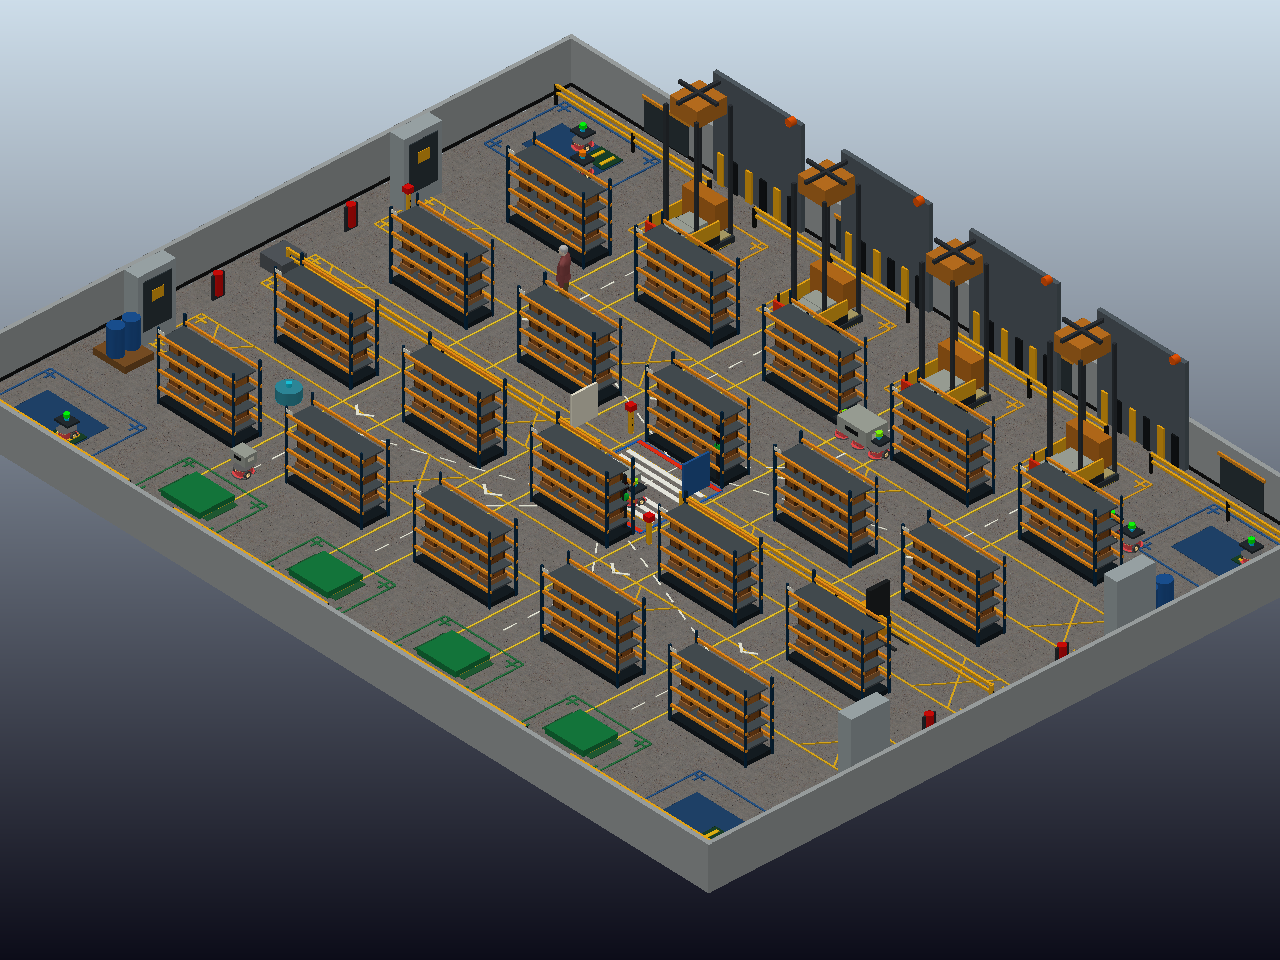
\includegraphics[width=0.76\textwidth]{figures/coppelia/aws-industrial-oblique-live.png}
    \caption{Montaje del almacén en CoppeliaSim. La vista oblicua muestra las
    estanterías, las zonas de operación, el paso central y la flota de AMR durante
    la ejecución del piloto.}
    \label{fig:method-coppeliasim-warehouse}
    \viusource{elaboración propia sobre la escena AWS RoboMaker Small Warehouse
    World, modificada para este TFM \parencite{awsRobomakerWarehouse2021}}
\end{figure}
\fi

La evidencia de CoppeliaSim se limita a la integración geométrica y al
\emph{replay} cinemático de estas interfaces. El agarre, la fricción
rueda--suelo, la dinámica de contacto y el comportamiento en hardware requieren
modelos y ensayos adicionales.

% Trasladado desde el capítulo 6 (enmienda de docs/02_RESEARCH_MATRIX.md,
% 2026-09-02): las Instrucciones VIU asignan a Metodología el diseño de
% investigación, las variables, los instrumentos y el análisis de datos, que
% es exactamente este material. Las etiquetas se conservan intactas para que
% las referencias cruzadas del capítulo 6 sigan resolviendo.
\subsection{Formulación general y arquitectura}
\label{subsec:common-formulation}

Sean \(\Robots\) los robots y \(\Loads\) las cargas. Para cada par \(i,k\), \(\boldsymbol c_i\) y \(\boldsymbol r_k\) representan capacidad y requisito, \(\rho_{ik}\) la preferencia y \(x_{ik}\) la pertenencia. Los costes estratégicos se expresan en escala normalizada; las variables físicas usan unidades SI.

La Tabla~\ref{tab:results-model-map} documenta qué etapa consulta agregados o cierres globales y cuál es su planta. Los códigos E0--E8 corresponden a los nombres históricos de las campañas \texttt{sp0}--\texttt{sp8}; no son subproblemas adicionales. El capítulo de resultados activa E2, E3, E4, E6, E7 y Cargo; E0, E1, E5 y E8 permanecen como procedencia y material de monografía, no como evidencia de una conclusión VIU.

\begin{table}[!htbp]
 \centering
 \caption{Contrato de distribución e interfaz física en las etapas experimentales de SP1--SP3.}
 \label{tab:results-model-map}
 \scriptsize
 \setlength{\tabcolsep}{2.2pt}
 \renewcommand{\arraystretch}{1.08}
 \begin{tabularx}{\textwidth}{@{}p{0.70cm}p{2.35cm}p{2.70cm}p{2.20cm}p{2.45cm}X@{}}
  \toprule
  Etapa & Decisión & Agregado o estimación & Cierre & Certificación & Planta \\
  \midrule
  E0 & revisión unilateral local & ocupación o precios globales; copias locales en el certificado auxiliar & discreto global & exclusividad & sin planta \\
  E1 & preferencia poblacional & cuotas globales & QR global & cardinalidad & sin planta \\
  E2 & ordenamiento secuencial & déficit global salvo la ablación primal--dual & global & umbral de servicio & sin planta \\
  E3 & pujas locales o vecinales parciales & residual exacto o consenso corto & global & QP de \emph{wrench} central & carga estática planar \\
  E4 & conflicto vecinal congelado & pose exacta de carga & bilateral/global & HOCBF y reparto de \emph{wrench} & uniciclo y carga planar en estratos separados \\
  E5 & coalición fija & geometría global filtrada por alcance & no aplica & filtro y reparto central por carga & cuerpo rígido planar \\
  E6 & marginal local & déficit publicado & local por carga & cobertura aditiva & viaje reducido \\
  E7 & ruta vecinal & intención local & testigo local & conflicto lógico visible & grafo discreto \\
  E8 & ruta vecinal & mensajes imperfectos & local & conflicto visible & grafo discreto; monografía \\
  Cargo & líder temporal tras \emph{gossip} de identificadores & atributos resueltos en registro global & líder por carga & criterio agregado, punto intermedio y filtro & uniciclo y carga planar en una misión \\
  \bottomrule
 \end{tabularx}
 \viuownsource
\end{table}

Una garantía puede pasar a la capa siguiente únicamente si esta conserva el estado, la información y el modelo de la prueba. Por ejemplo, la cobertura nominal de recursos debe someterse todavía al certificado de contacto antes de salir de SP1. En Cargo, los enlaces vecinales descubren identificadores; el ejecutor consulta estado global para elegir líder y resolver atributos. Su admisión inicial usa un criterio agregado distinto del QP de la etapa E3. Estas dependencias hacen híbrida la arquitectura.


\subsection{Protocolo común y métodos de referencia}
\label{subsec:common-protocol}

Cada celda experimental reutiliza el mundo y la semilla entre métodos, con idénticos límites de actuación, horizonte y criterio de éxito. Las colisiones, los bloqueos y los agotamientos del horizonte permanecen en el denominador. Las tablas distinguen el oráculo con información global del método, los comparadores y las ablaciones. La clase de complejidad corresponde al problema; el tiempo o la cota informados corresponden al algoritmo ejecutado.

Las etapas E2--E4 son reanálisis de observaciones archivadas, con postproceso, tablas y auditorías disponibles. Parte de sus generadores históricos falta. Cargo sí puede regenerarse desde su configuración y reproduce el demostrador híbrido implementado; esta campaña no ejecuta la composición exacta de los mecanismos parciales de SP1 y SP2.

\subsection{Criterios de comparación}
\label{subsec:method-comparison}

La Tabla~\ref{tab:tf-comparison} clasifica la salida que cada familia entrega a
la capa siguiente. ``Parcial'' indica que la propiedad depende de un módulo o
de supuestos externos al problema tratado.

\begin{table}[!htbp]
  \centering
  \caption{Cobertura de las familias metodológicas relevantes.}
  \label{tab:tf-comparison}
  \scriptsize
  \setlength{\tabcolsep}{2.4pt}
  \begin{tabularx}{\textwidth}{@{}p{2.0cm}p{1.25cm}p{1.35cm}p{1.45cm}X p{2.2cm}@{}}
    \toprule
    Familia & Coalición & Física & Información local & Garantía típica & Límite para este problema \\
    \midrule
    Asignación/MILP & Sí & Parcial & No & óptimo o cota del optimizador & coste global y combinatorio \\
    Subasta/CBBA & Parcial & No & Sí & asignación bajo supuestos de puntuación y red & no certifica contacto \\
    Juego de coalición & Sí & Parcial & Sí & estabilidad o mejora local & no implica óptimo social \\
    Juego poblacional & Relajada & No & Parcial & convergencia bajo estructura del juego & exige cierre entero \\
    Consenso/primal--dual & No & No & Sí & acuerdo o convergencia bajo red y regularidad & no decide ni estabiliza la planta \\
    Formación/\emph{wrench} & Equipo dado & Sí & Parcial & rigidez, reparto o seguimiento & no selecciona el equipo \\
    ORCA/CBF & No & Parcial & Sí & evitación o invariancia condicionada & puede bloquearse \\
    Reparación por evento & Parcial & No & Sí & reasignación o activación alternativa & exige recertificar la coalición \\
    MAPF/tráfico & No & Huella parcial & Parcial & completitud, optimalidad o cota según método & conflicto discreto no es colisión física \\
    MARL/GNN & Aprendida & Parcial & Sí & rendimiento empírico & interpretación y garantías limitadas \\
    \bottomrule
  \end{tabularx}
  \viuownsource
\end{table}

Las familias parten de objetos distintos: asignación consume utilidad, formación
consume un equipo, seguridad consume un control nominal y MAPF una abstracción
espacio--temporal. En instancias pequeñas, el oráculo global fija un techo bajo
información privilegiada; la brecha, la comunicación y la conectividad se miden
por separado. El oráculo no se presenta como competidor distribuido.

Con restricciones compartidas y las condiciones de regularidad declaradas, un
Nash generalizado variacional se caracteriza como solución de una desigualdad
variacional y admite multiplicadores comunes
\parencite{yi2019operatorGNE,franci2022stochasticGNE}. Las dinámicas
primal--dual actualizan esos multiplicadores junto con las decisiones bajo
convexidad, monotonicidad y conectividad
\parencite{cherukuri2016primalDual,koshal2016aggregative}. El precio dual
representa congestión o déficit; la integralidad y el coste social requieren
mecanismos y estimandos separados.

El protocolo exige que una prueba de pasividad identifique puertos,
almacenamiento y suministro, y que una prueba de Lyapunov fije dominio y signo
de la derivada \parencite{vanderschaf2017passivity,ortega2002passivity}. Un
cambio de contacto, la saturación o la discretización alteran esas hipótesis.
La interconexión híbrida necesita una prueba composicional incluso si la capa
estratégica y la planta poseen resultados locales propios.

